\documentclass[12pt, dvipsnames, a4paper]{article}
\usepackage{geometry}
\geometry{legalpaper, margin=0.5in}
\usepackage{xcolor}
\usepackage{lipsum,etoolbox}
\usepackage{xspace} 
\usepackage[normalem]{ulem}
\usepackage{vwcol}
\usepackage{cancel}
\usepackage{enumitem}
\usepackage{amsmath}
\usepackage{caption}
\usepackage{graphicx}
\usepackage{amsfonts}
\usepackage{float}
\usepackage{multicol}
\usepackage{hyperref}
\usepackage{listings}
\usepackage{textcomp}
\usepackage{lstautogobble}
\usepackage[parfill]{parskip}
\usepackage{tikz-qtree}
\usepackage{tikz}
\usepackage{hyperref}
\usetikzlibrary{decorations.pathreplacing}
\tikzset{every tree node/.style={minimum width=4cm,draw,circle},
         blank/.style={draw=none},
         edge from parent/.style=
         {draw,edge from parent path={(\tikzparentnode) -- (\tikzchildnode)}},
         level distance=1.5cm}

%% Genearl %%
\renewcommand{\thesection}{\arabic{section}}


%% For convenience %%
\newcommand{\code}[1]{\texttt{#1}}
\newcommand{\bcode}[1]{\texttt{\textbf{#1}}}
\newcommand{\balert}[1]{\textbf{\alert{#1}}}
\newcommand{\rarrow}{$\Rightarrow$}
\newcommand{\tab}[1][0.5cm]{\hspace*{#1}}
\newcommand{\deepemphasis}[1]{\underline{\textbf{\Large{#1}}}}
\newcommand{\bfemph}[1]{\textbf{\emph{#1}}}
\newcommand{\OR}[0]{\lvert \: \rvert}

%% Colours %%
\definecolor{mLightBrown}{HTML}{EB811B}
\definecolor{mLightGreen}{HTML}{14B03D}

%% Pseudocode %% 
\lstdefinelanguage{pseudo}
{
	keywords=[1]{
		let,
		class,
		new,
		loop,
		until,
		end,
		if,
		else,
		then,
		return,
		while,
		for,
		to,
		fun,
		break,
		and,
		true,
		false,
		or,
		do,
		max,
		min,
		elif,
	},
	keywordstyle=[1]\color{black}\bf,
	keywords=[2] {
		invariant,
		precond,
		postcond
	},
	keywordstyle=[2]\color{blue}\bf
}

\lstset{
	breaklines		=	true,
	language 		= 	pseudo,
	basicstyle		=	\ttfamily,
	mathescape		=	true,
	escapeinside	=	||,
	tabsize			=	2,
	numbers			=	left,
	commentstyle	=	\color{OliveGreen},
	stringstyle		=	\color{mLightBrown},
	upquote			=	true,
	morestring		=	[b]',
	moredelim		=	[l][\rmfamily\itshape]{@},
	comment			=	[l]{//},
	morecomment		=	[s]{/*}{*/},
	commentstyle=\color{Gray}\ttfamily,
	showstringspaces=	false,
	showtabs		=	false,
	autogobble
}

%% Other %%
\setcounter{secnumdepth}{5}
\setcounter{tocdepth}{5}

% \patchcmd{<cmd>}{<search>}{<replace>}{<success>}{<failure>}
\patchcmd{\abstract}{\titlepage}{\titlepage% Insert ToC-writing after starting a titlepage
  \addcontentsline{toc}{chapter}{Abstract}}{}{}
\setcounter{secnumdepth}{3}
\setcounter{tocdepth}{3}

% Keywords command
\providecommand{\keywords}[1]
{
  \small	
  \textbf{\textit{Keywords---}} #1
}


%**************************************************************************************************************%
%______________________________________________________________________________________________________________%
\begin{document}
\title{\textbf{EECS 4314 - Bit Theory\\Concrete Architecture Report}}
\date{\Large \today}
\author{
	\large \textbf{Amir Mohamad}\\ \small amohamad@my.yorku.ca\\\\
	\large \textbf{Arian Mohamad Hosaini}\\ \small mohama23@my.yorku.ca\\\\
	\large \textbf{Dante Laviolette}\\ \small dantelav@my.yorku.ca\\\\
	\large \textbf{Diego Santosuosso Salerno}\\ \small nicodemo@my.yorku.ca\\\\
	\large \textbf{Isaiah Linares}\\ \small isaiah88@my.yorku.ca\\\\
	\large \textbf{Joel Fagen}\\ \small joefagan@my.yorku.ca\\\\
	\large \textbf{Misato Shimizu}\\ \small misato1@my.yorku.ca\\\\
	\large \textbf{Muhammad Hassan}\\ \small furquanh@my.yorku.ca\\\\
	\large \textbf{Yi Qin}\\ \small aidenqin@my.yorku.ca\\\\
	\large \textbf{Zhilong Lin}\\ \small lzl1114@my.yorku.ca\\\\
	\large York University\\
}
\maketitle
\newpage
\hspace{0pt}
\vfill
\begin{abstract}
	\lipsum[1]
	\lipsum[1]
	\\\\
	\keywords{keyword1, keyword2, keyword3}
\end{abstract}
\vfill
\hspace{0pt}
\newpage
\tableofcontents
\clearpage

\section{Introduction}
\lipsum[1]

\subsection{Overview}
\lipsum[1]

\section{Architecture}
\lipsum[1]

\section{Diagrams}
\lipsum[1]

\section{External Interfaces}
\lipsum[1]

\section{Use Cases}
\subsection{Piping In Shell}
The following sequence diagram shows how system calls can be used to pipe the
output of 1 application to the input of another in FreeBSD, using a shell
as an example program.
\begin{figure}[!htb]
	\advance\leftskip-0.5cm
	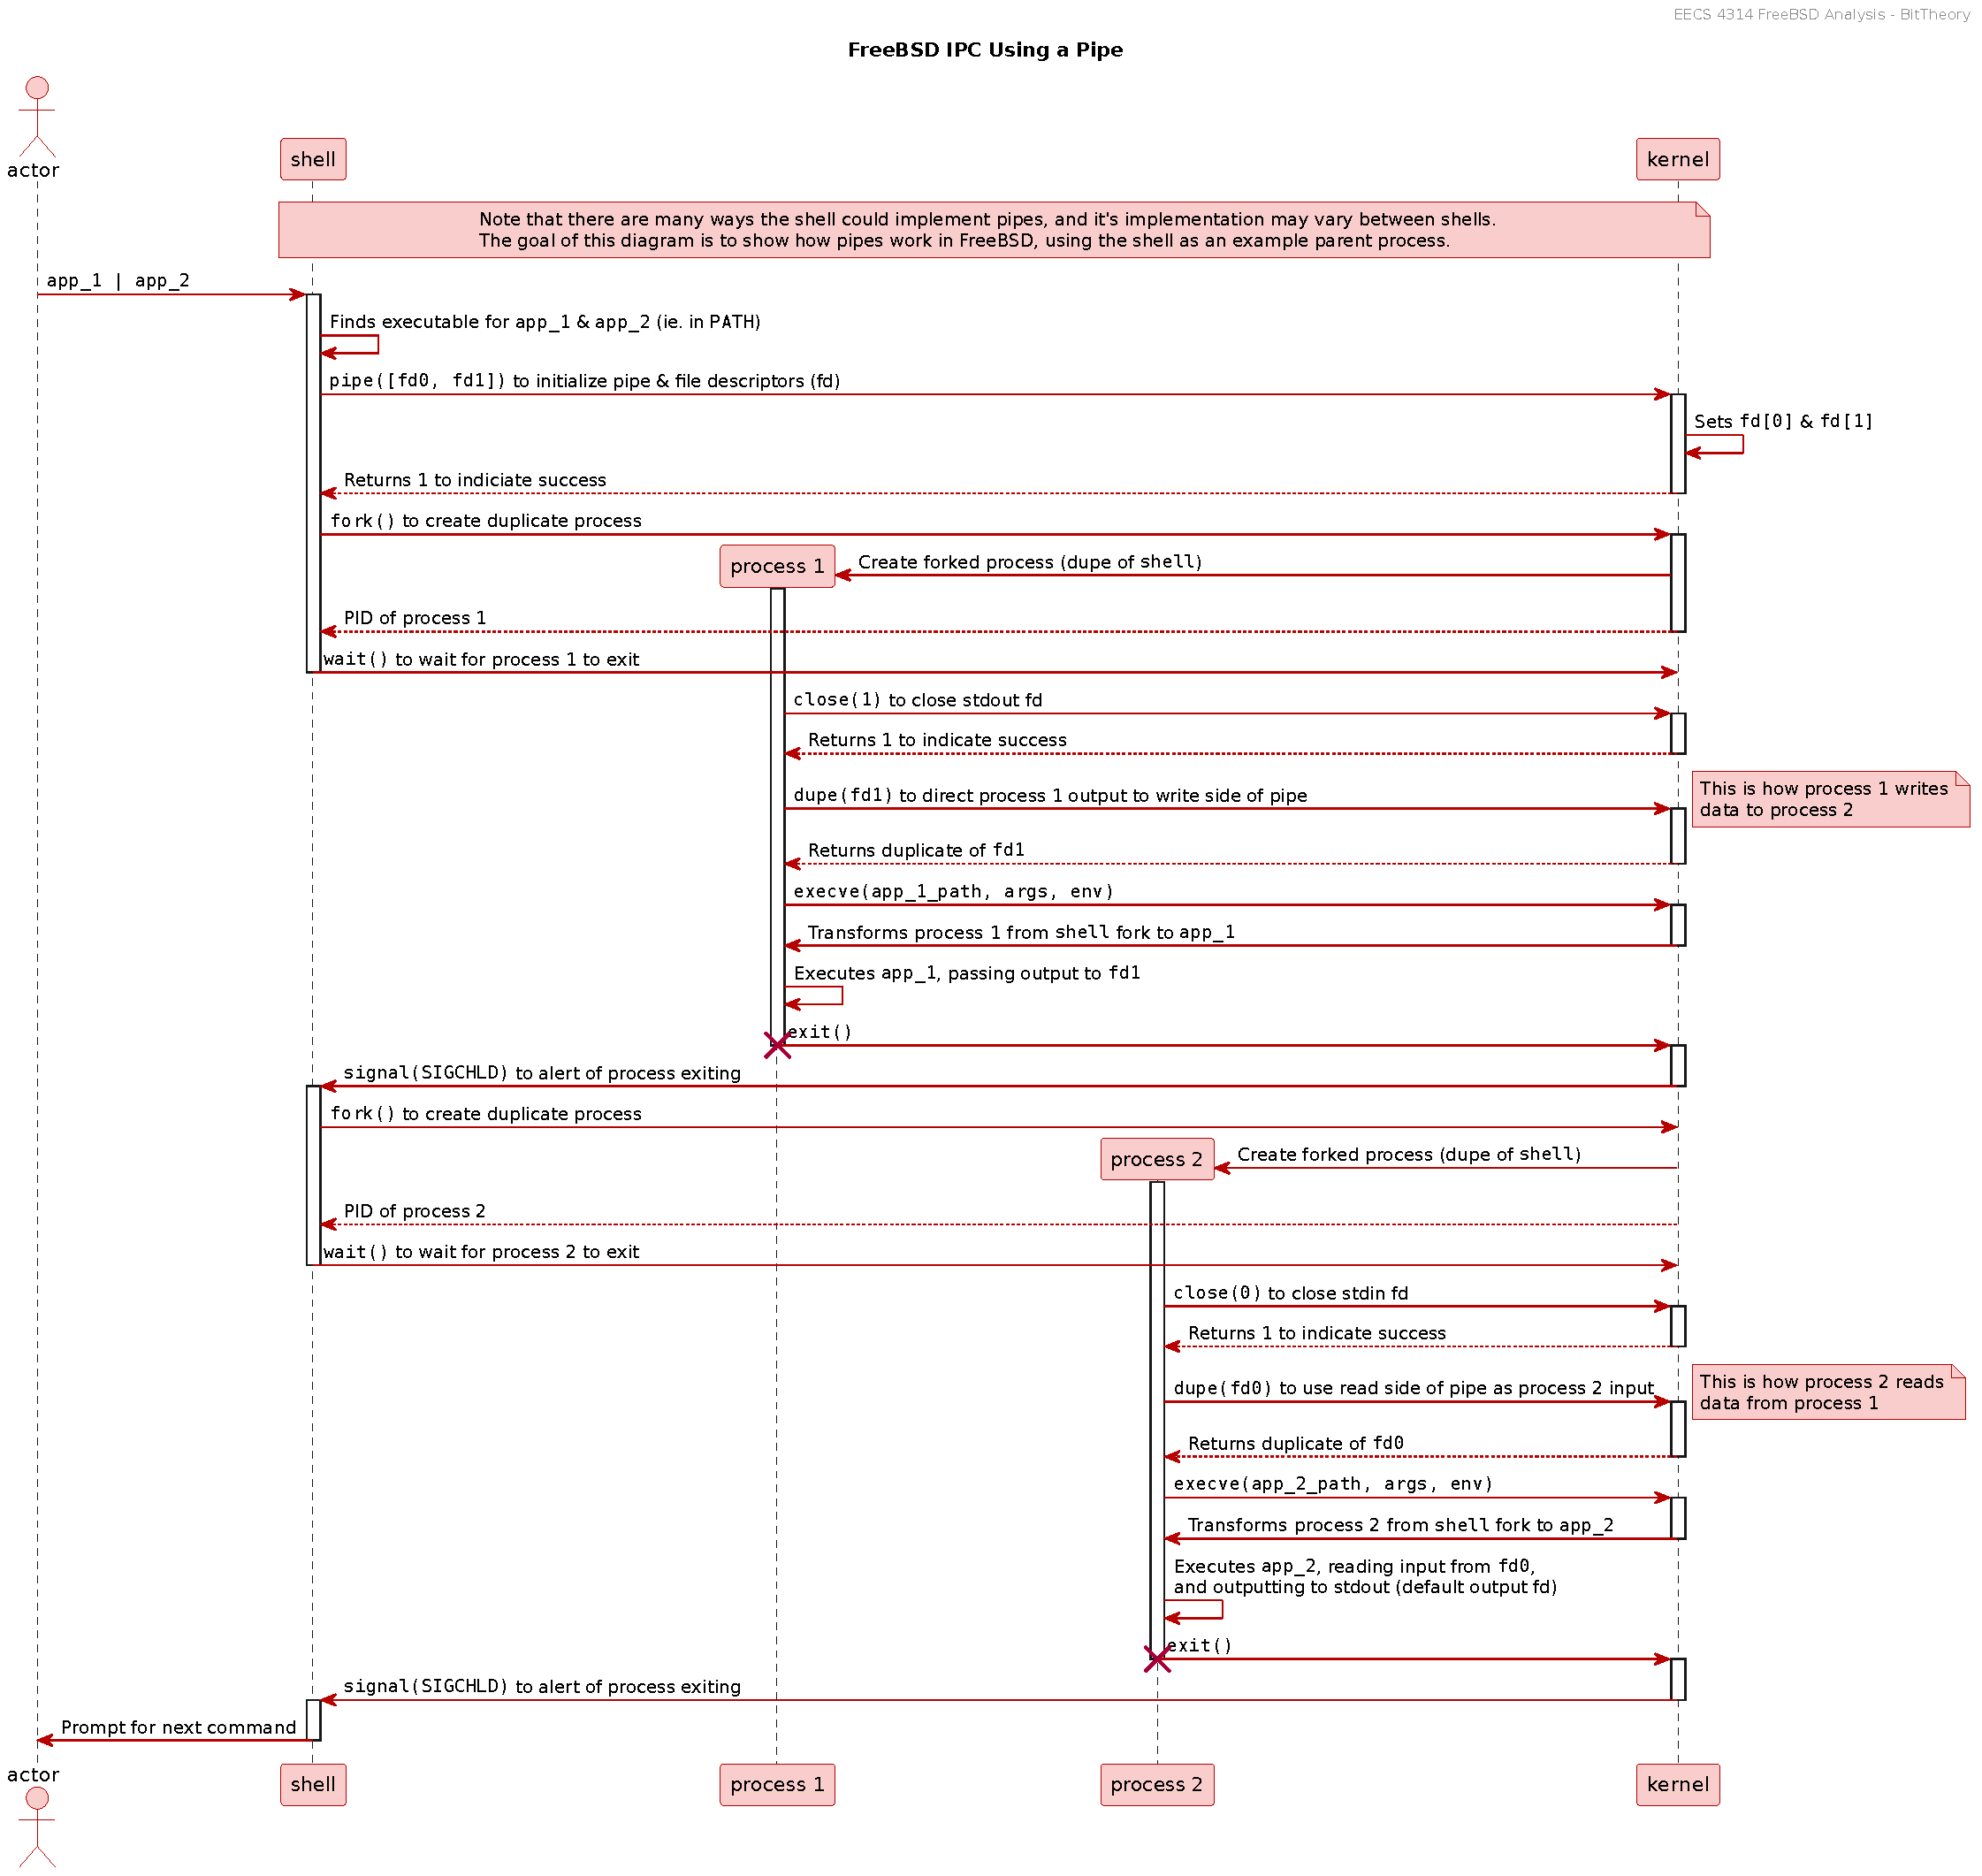
\includegraphics[width = 570pt]{assets/use_case_diagrams/pipe.pdf}
	\caption{Sequence diagram showing pipes being used in the shell for IPC. \cite{pipe}\cite{fork}\cite{wait}\cite{close}\cite{dup}\cite{execve}\cite{signal}\cite{pipe-explained}}
\end{figure}
\clearpage

\section{Data Dictionary}
\lipsum[1]

\section{Naming Conventions}
\lipsum[1]

\section{Conclusion}
\lipsum[1]

\section{Lessons Learned}
\lipsum[1]

\begin{thebibliography}{00}
	\bibitem{pipe} “FreeBSD Manual Pages.” Pipe(2), \href{https://man.freebsd.org/cgi/man.cgi?pipe\%282\%29}{https://man.freebsd.org/cgi/man.cgi?pipe\%282\%29}.
	\bibitem{fork} “FreeBSD Manual Pages.” Fork(2), \href{https://man.freebsd.org/cgi/man.cgi?fork(2)}{https://man.freebsd.org/cgi/man.cgi?fork(2)}.
	\bibitem{wait} “FreeBSD Manual Pages.” Wait(2), \href{https://man.freebsd.org/cgi/man.cgi?wait(2)}{https://man.freebsd.org/cgi/man.cgi?wait(2)}.
	\bibitem{close} “FreeBSD Manual Pages.” Close(2), \href{https://man.freebsd.org/cgi/man.cgi?query=close\&sektion=2}{https://man.freebsd.org/cgi/man.cgi?query=close\&sektion=2}.
	\bibitem{dup} “FreeBSD Manual Pages.” Dup(2), \href{https://man.freebsd.org/cgi/man.cgi?query=dup\&sektion=2\&n=1}{https://man.freebsd.org/cgi/man.cgi?query=dup\&sektion=2\&n=1}.
	\bibitem{execve} “FreeBSD Manual Pages.” Execve(2), \href{https://man.freebsd.org/cgi/man.cgi?query=execve\&sektion=2\&n=1}{https://man.freebsd.org/cgi/man.cgi?query=execve\&sektion=2\&n=1}.
	\bibitem{signal} “FreeBSD Manual Pages.” Signal(3), \href{https://man.freebsd.org/cgi/man.cgi?sektion=3\&query=signal}{https://man.freebsd.org/cgi/man.cgi?sektion=3\&query=signal}.
	\bibitem{pipe-explained} Menon-Sen, Abhijit. “How Are Unix Pipes Implemented?” Toroid.org, 27 Mar. 2020, \href{https://toroid.org/unix-pipe-implementation}{https://toroid.org/unix-pipe-implementation}.
\end{thebibliography}
\end{document}
